\documentclass[tikz,border=6pt]{standalone}

% общий стиль (подключается через TEXINPUTS)
% tikz-style.tex (общий стиль для всех TikZ-картинок)
\RequirePackage[T1,T2A]{fontenc}
\RequirePackage[utf8]{inputenc}

% Palatino-подобный шрифт (как в MathJax часто воспринимается «более вытянутым»)
\RequirePackage{txfonts}
% txfonts даёт предупреждение по кириллице (T2A/txr не определён).
% Оставляем txfonts для математики, а текстовый шрифт возвращаем на Computer Modern,
% чтобы не искать T2A/txr и убрать предупреждения.
\renewcommand{\rmdefault}{cmr}
\renewcommand{\sfdefault}{cmss}
\renewcommand{\ttdefault}{cmtt}

\RequirePackage{tikz}
\RequirePackage{xcolor}
\usetikzlibrary{calc}

% цвета
\definecolor{lightgreen}{RGB}{214,234,214}
\definecolor{darkgreen}{HTML}{0B7A0B}
\definecolor{darkred}{HTML}{DF0000}

\definecolor{midgreen}{HTML}{2E9B2E}
\definecolor{palegreen}{RGB}{235,246,235}
\definecolor{olivegreen}{HTML}{3E6B2F}

\definecolor{lightred}{RGB}{255,220,220}
\definecolor{midred}{HTML}{E04545}
\definecolor{darkred2}{HTML}{A80000}

\definecolor{lightblue}{RGB}{220,232,255}
\definecolor{midblue}{HTML}{2E5BD6}
\definecolor{darkblue}{HTML}{0B2E8A}

\definecolor{lightgray}{RGB}{240,240,240}
\definecolor{midgray}{RGB}{170,170,170}
\definecolor{darkgray}{RGB}{80,80,80}

\definecolor{vtxfill}{RGB}{86,193,255}
\definecolor{vennfill}{RGB}{220,232,255}


% единый набор стилей TikZ
\tikzset{
    lab/.style={
        font=\fontsize{24}{32}\selectfont
    }
}


\begin{document}
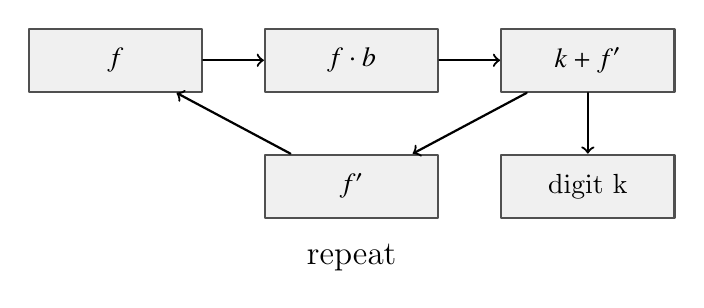
\begin{tikzpicture}[x=1cm,y=1cm, line cap=round, line join=round]

\tikzset{
  box/.style={draw=darkgray, fill=lightgray, line width=0.8pt, minimum width=2.2cm, minimum height=0.8cm},
  lab/.style={font=\large}
}

\node[box] (f0) at (0,0) {$f$};
\node[box] (mul) at (3,0) {$f \cdot b$};
\node[box] (split) at (6,0) {$k + f'$};

\node[box] (digit) at (6,-1.6) {digit k};
\node[box] (f1) at (3,-1.6) {$f'$};

\draw[->, line width=0.8pt] (f0) -- (mul);
\draw[->, line width=0.8pt] (mul) -- (split);
\draw[->, line width=0.8pt] (split) -- (digit);
\draw[->, line width=0.8pt] (split) -- (f1);
\draw[->, line width=0.8pt] (f1) -- (f0);

\node[lab] at (3,-2.5) {repeat};

\end{tikzpicture}
\end{document}
